\documentclass[12pt]{article}
\usepackage[T1]{fontenc}
\usepackage[polish]{babel}
\usepackage[utf8]{inputenc}
\usepackage{graphicx}

% *** KLUCZOWA ZMIANA TUTAJ ***
% Ładujemy listings z opcją [table] i umieszczamy definicje zaraz za nim.
\usepackage{listings}
\makeatletter
\def\l@lstlisting{\@dottedtocline{1}{1.5em}{2.3em}}
\makeatother
% *** KONIEC KLUCZOWEJ ZMIANY ***

\usepackage{float}
\usepackage{xcolor}
\usepackage[left=2cm,right=2cm,top=2cm,bottom=2cm]{geometry}
% Hyperref powinien być ZAWSZE jednym z ostatnich pakietów
\usepackage[colorlinks=true, linkcolor=blue]{hyperref}
\renewcommand{\lstlistlistingname}{Spis listingów}
\hypersetup{linktoc=page}

% Reszta Twoich definicji kolorów i języków listings...
% Tutaj powinieneś zachować wszystkie \definecolor, \lstdefinelanguage, \lstdefinestyle, \lstset

% Define colors for the listing (optional, but makes it look better)
\definecolor{codegray}{rgb}{0.5,0.5,0.5}
\definecolor{backcolor}{rgb}{0.98,0.98,0.98}
\definecolor{keywords}{rgb}{0,0,1}
\definecolor{comments}{rgb}{0,0.5,0}
\definecolor{strings}{rgb}{0.6,0,0}

\lstdefinelanguage{JavaScript}{
	keywords={function, var, return, if, else, for, while, do, break, continue, switch, case, default, new, try, catch, finally, throw, this, typeof, instanceof, in, with, class, const, let, export, import, async, await},
	morecomment=[l]{//},
	morecomment=[s]{/*}{*/},
	morestring=[b]",
	morestring=[b]',
	sensitive=false,
	moredelim=[s][\color{keywords}]{<}{>},
}

% Define the HTML language
\lstdefinelanguage{HTML5}{
	sensitive=true,
	keywords={html,head,title,body,div,span,h1,h2,h3,p,a,section,article,footer,nav},
	morekeywords=[2]{class,style,lang,data-stellar-background-ratio,id,src,alt}, % Atrybuty HTML
	morekeywords=[3]{th:block,th:text,th:href,th:replace,th:each,th:if,th:unless}, % Atrybuty Thymeleaf
	morestring=[b]{"},
	morestring=[b]{'},
	morecomment=[s]{}, % Zmieniono z {} na prawidłowe delimitery HTML
	moredelim=[s][\color{codepurple}]{<}{>}, % To podświetli tagi HTML
	alsoletter={:,-} % Obsługa dwukropków w Thymeleaf i myślników w atrybutach data-*
}

\lstdefinestyle{jsStyle}{
	language=JavaScript,
	backgroundcolor=\color{backcolor},
	basicstyle=\ttfamily\footnotesize,
	keywordstyle=\color{keywords}\bfseries,
	commentstyle=\color{comments},
	stringstyle=\color{strings},
	numberstyle=\tiny\color{codegray},
	numbers=left,
	numbersep=5pt,
	breaklines=true,
	frame=single,
	tabsize=2
}

\lstset{
	backgroundcolor=\color{backcolor},
	commentstyle=\color{comments},
	keywordstyle=\color{keywords},
	numberstyle=\tiny\color{codegray},
	stringstyle=\color{strings},
	basicstyle=\ttfamily\footnotesize,
	breakatwhitespace=false,
	breaklines=true,
	captionpos=b,
	keepspaces=true,
	numbers=left,
	numbersep=5pt,
	showspaces=false,
	showstringspaces=false,
	showtabs=false,
	tabsize=2,
	title=\lstname,
	frame=single,
	rulesepcolor=\color{gray},
	identifierstyle=\color{black},
}

\lstdefinestyle{customjava}{
	language=Java,
	basicstyle=\ttfamily\small,
	keywordstyle=\color{blue}\bfseries,
	commentstyle=\color{gray},
	stringstyle=\color{teal},
	numbers=left,
	numberstyle=\tiny\color{gray},
	stepnumber=1,
	numbersep=5pt,
	backgroundcolor=\color{white},
	frame=single,
	rulecolor=\color{black},
	tabsize=2,
	captionpos=b,
	breaklines=true,
	breakatwhitespace=true,
	showstringspaces=false
}

% Define the CSS language
\lstdefinelanguage{CSS}{
	keywords={%
		% Selectors
		html, article, aside, figcaption, figure, footer, header, hgroup, main, nav, section, body,%
		% Properties
		font-family, line-height, -webkit-text-size-adjust, -webkit-tap-highlight-color, display, margin, font-size, font-weight, color, text-align, background-color%
	},
	morecomment=[l]{//},
	morecomment=[s]{/*}{*/},
	string=[b]",
	string=[b]',
	sensitive=false,
	classoffset=1, % For pseudo-classes/elements if needed
	morekeywords={%
		% Pseudo-classes/elements (example, add more as needed)
		:hover, :active, :focus, ::before, ::after%
	},
	classoffset=0,
}

% Set up common listing styles (optional, but good practice)
\lstset{
	backgroundcolor=\color{backcolor},
	commentstyle=\color{green!50!black},
	keywordstyle=\color{blue},
	numberstyle=\tiny\color{codegray},
	stringstyle=\color{red},
	basicstyle=\ttfamily\footnotesize,
	breakatwhitespace=false,
	breaklines=true,
	captionpos=b,
	keepspaces=true,
	numbers=left,
	numbersep=5pt,
	showspaces=false,
	showstringspaces=false,
	showtabs=false,
	tabsize=2,
	title=\lstname,
	frame=single,
	rulesepcolor=\color{gray},
	identifierstyle=\color{black},
}

%opening
\title{Dokumentacja aplikacji InstaCar}
\author{Sebastian Górski\\ Jakub Grzymisławski\\ Łukasz Szenkiel}
\date{}


\begin{document}
	
	\maketitle
	\thispagestyle{empty} 
	
	\begin{center}
		\vspace{10em}
		
\includegraphics[width=0.6\textwidth]{CWUPlogo.png} \\[10em]
	\end{center}
	
	\newpage
	\tableofcontents
	
	\newpage
\section*{Opis}
\addcontentsline{toc}{section}{Opis}

Dokumentacja dotyczy aplikacji \textit{InstaCar}, nowoczesnego systemu służącego do rezerwacji samochodów na wynajem. Aplikacja umożliwia użytkownikom przeglądanie dostępnych pojazdów, filtrowanie wyników według, daty, ceny i rodzaju pojazdu, a następnie dokonywanie rezerwacji w wybranym terminie. Zarejestrowani użytkownicy mają również możliwość zarządzania swoimi rezerwacjami.\\
\textit{InstaCar} została zaprojektowana z myślą o wygodzie użytkownika i łatwej skalowalności. Interfejs użytkownika jest responsywny i intuicyjny, dostosowany zarówno do urządzeń mobilnych, jak i komputerów stacjonarnych. Aplikacja wykorzystuje nowoczesne technologie frontendowe oraz bezpieczne mechanizmy logowania i autoryzacji. System wspiera również funkcjonalności takie jak powiadomienia e-mail o dokonaniu rezerwacji.\\
Dokumentacja zawiera szczegółowy opis funkcjonalności systemu, architektury aplikacji, instrukcję użytkowania, wymagania techniczne oraz informacje przeznaczone dla administratorów i deweloperów. Uwzględniono również aspekty związane z bezpieczeństwem, testowaniem oraz możliwością dalszego rozwoju aplikacji.

	
\newpage
\section{Architektura systemu}
W tej sekcji przedstawiono opis architektury systemu \textit{Instacar}.
	
\subsection{Diagram czynności}
	Diagram czynności ilustruje przebieg głównych procesów w aplikacji, takich jak rezerwacja pojazdu czy logowanie użytkownika.
	\begin{figure}[H]
		\centering
		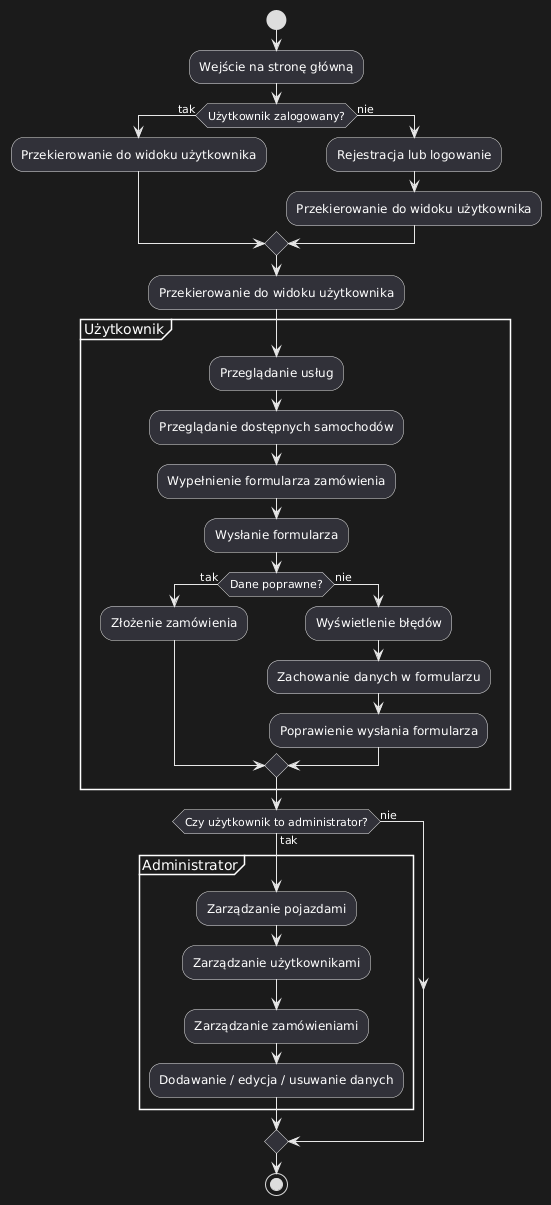
\includegraphics[height=0.78\textheight]{diagramCzynnosci}
		\caption{Diagram czynności}
		\label{fig:diagramCzynnosci}
	\end{figure}
	
\subsection{Diagram kluczowych klas}
	Diagram klas przedstawia strukturę aplikacji \textit{InstaCar} w ujęciu obiektowym, wraz z zależnościami między klasami.
	
	\begin{figure}[H]
		\centering
		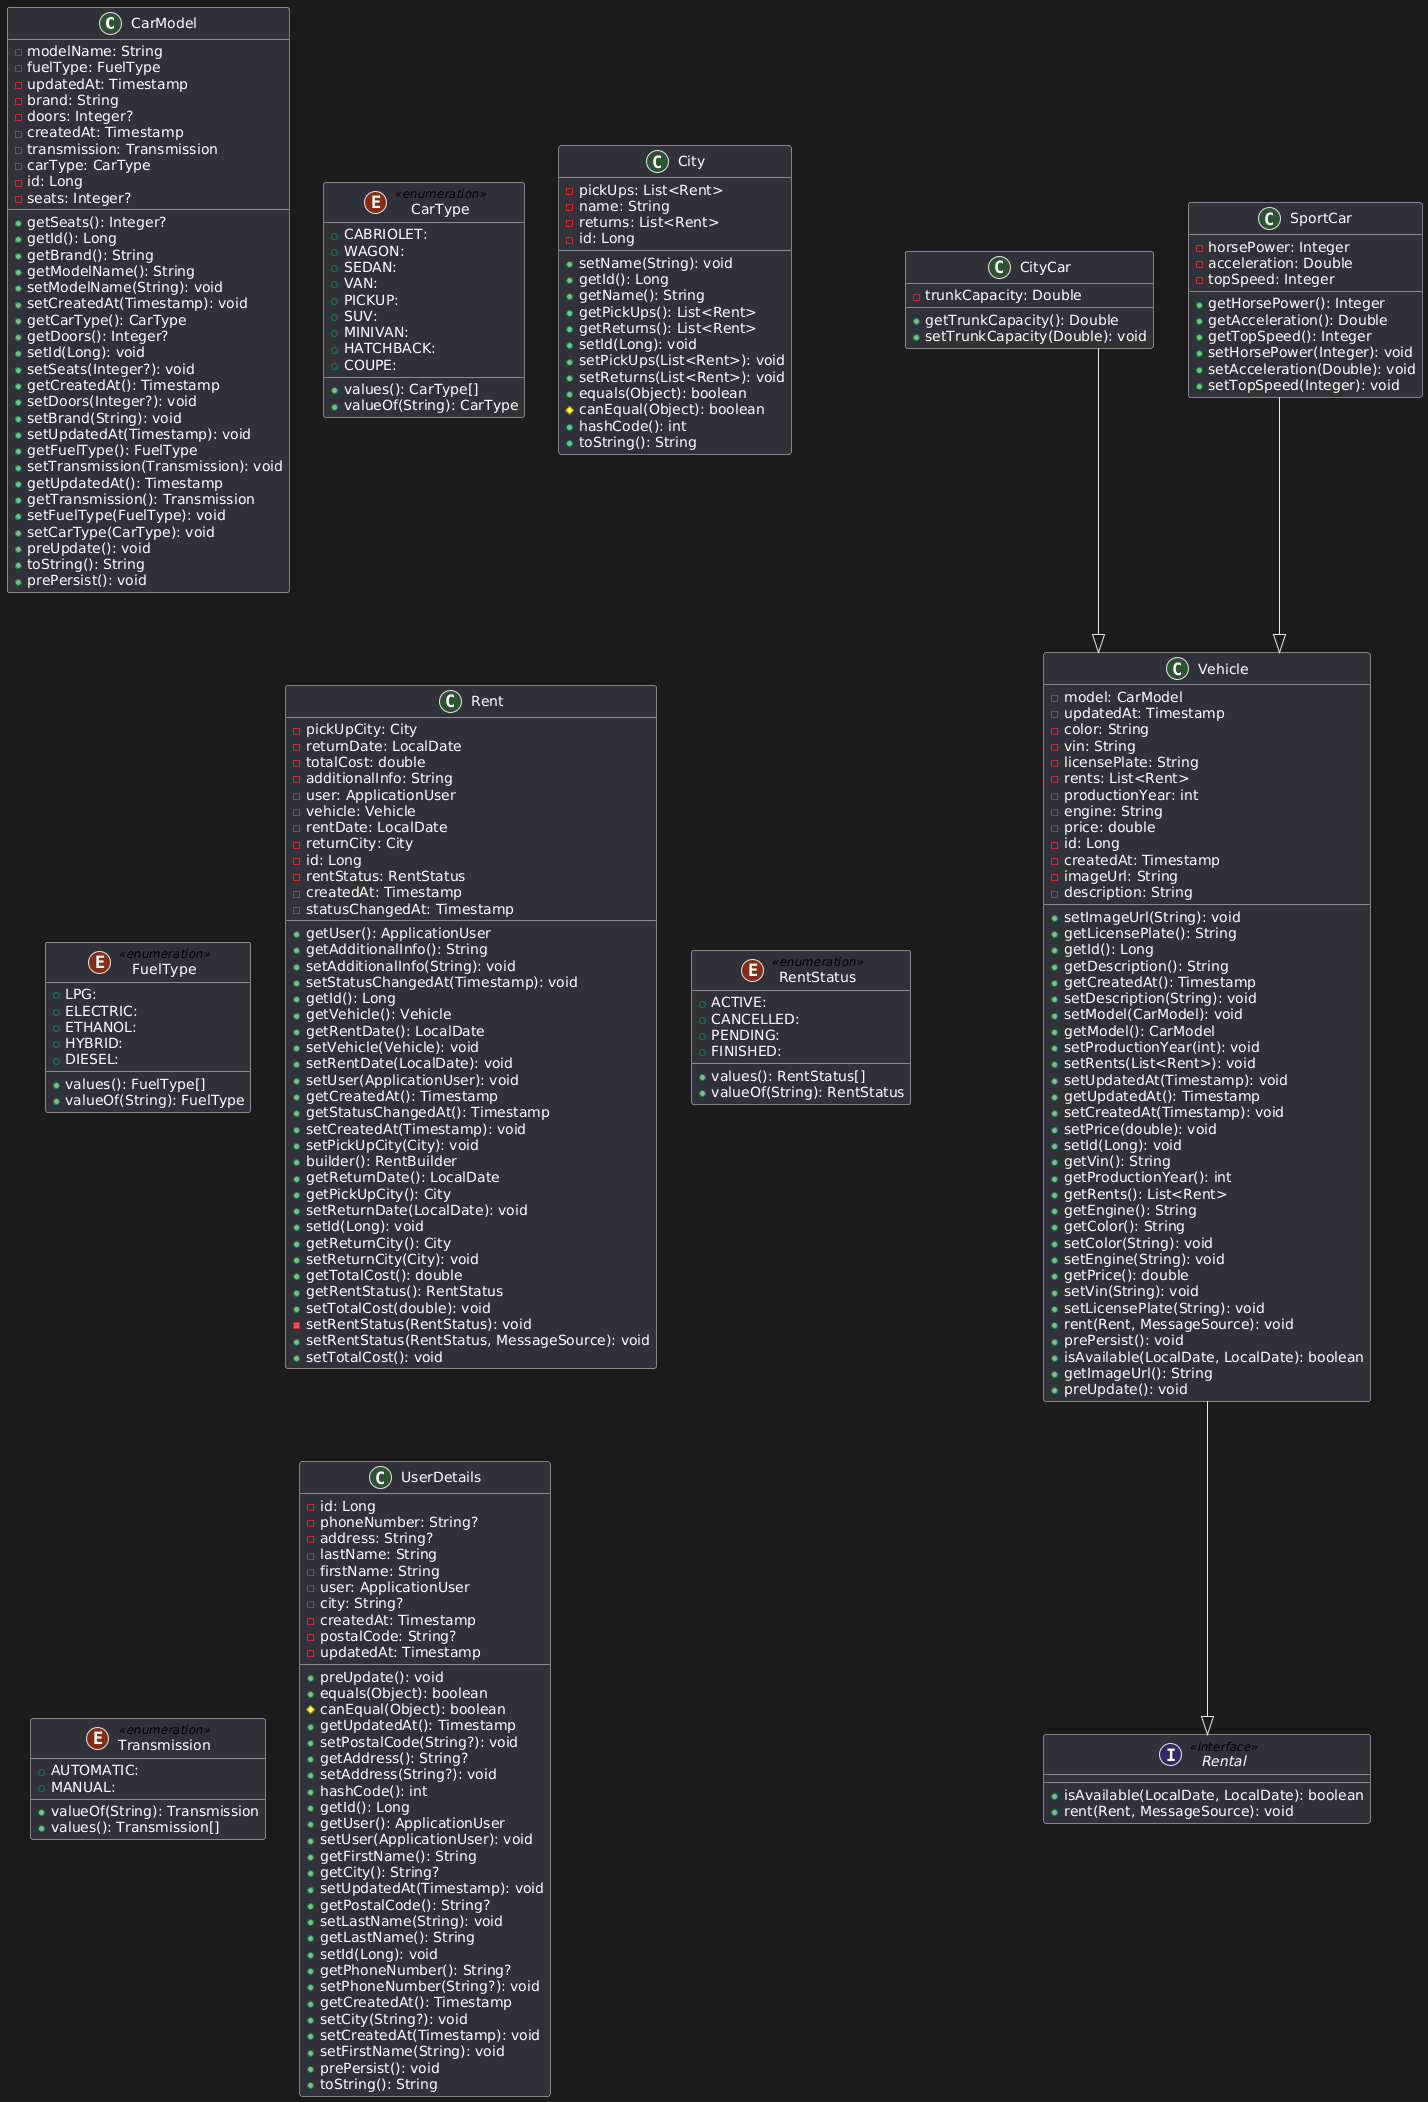
\includegraphics[width=1\linewidth, height=0.84\textheight]{diagramKlas}
		\caption{Diagram klas}
		\label{fig:diagramklas}
	\end{figure}
	
	\newpage
	\subsection{Diagram encji}
	Diagram encji przedstawia strukturę bazy danych systemu wypożyczalni pojazdów, uwzględniając tabele użytkowników, pojazdów, wynajmów oraz relacje między nimi.
	
	\begin{figure}[H]
		\centering
		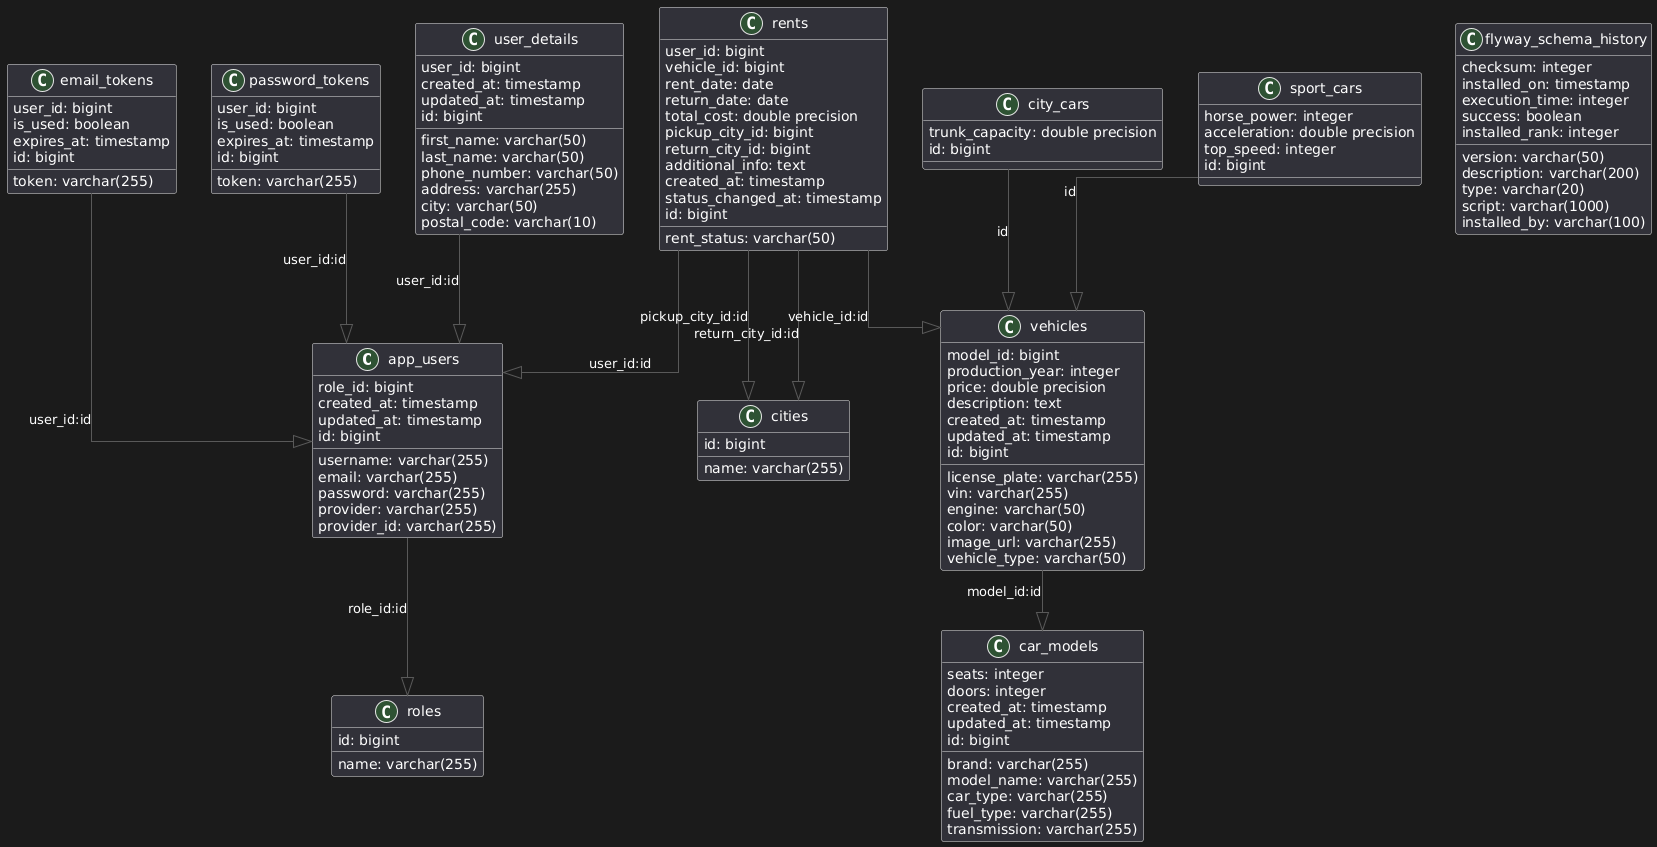
\includegraphics[width=1\linewidth]{diagram_bd}
		\caption{Diagram encji bazy danych}
		\label{fig:diagram_bd.png}
	\end{figure}
	
	\newpage
	\subsection{Diagram przypadków użycia}
	Diagram przypadków użycia ukazuje interakcje użytkowników z systemem, identyfikując główne funkcje dostępne w aplikacji.
	
	\begin{figure}[H]
		\centering
		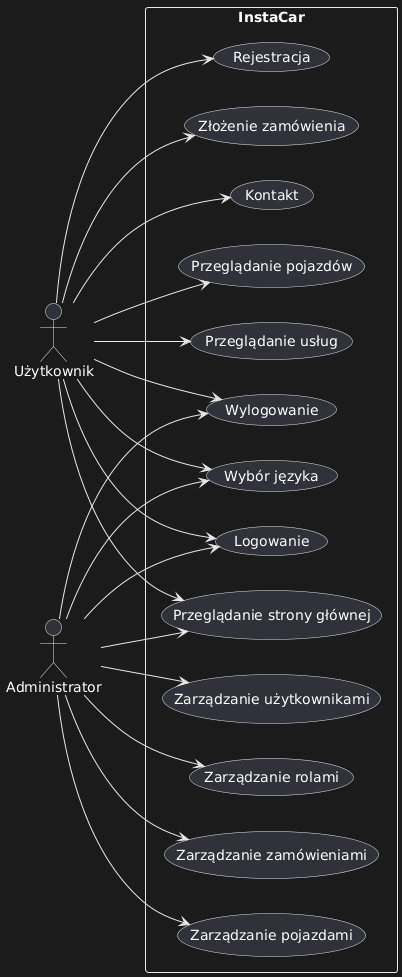
\includegraphics[height=0.78\textheight]{diagramPrzypadkowUzycia}
		\caption{Diagram przypadków użycia}
		\label{fig:diagramPrzypadkowUzycia}
	\end{figure}
	
\subsection{Implementacja kodu}
Aplikacja \textit{InstaCar} została zaimplementowana z wykorzystaniem frameworka Spring Boot, który ułatwia tworzenie aplikacji webowych w języku Java. Projekt został zorganizowany zgodnie z~architekturą MVC (Model-View-Controller), co zapewnia czytelność i separację odpowiedzialności w~kodzie.

\subsubsection{Stos technologiczny}
\begin{itemize}
	\item \textbf{Backend}: Java 21, Spring Boot, Spring Data JPA, Spring Security
	\item \textbf{Frontend}: HTML, CSS, Thymeleaf
	\item \textbf{Baza danych}: PostgreSQL, Redis 7.4.2-alpine
	\item \textbf{Zarządzanie projektem}: Maven
\end{itemize}

\subsubsection{Widoki i formularze}
Do tworzenia warstwy prezentacji wykorzystano szablony Thymeleaf, które integrują się bezpośrednio ze Spring Boot. Formularze użytkownika przesyłają dane do kontrolerów, gdzie są one poddawane walidacji. W przypadku błędów formularz zostaje ponownie załadowany z zachowaniem wcześniej wpisanych danych oraz komunikatami o nieprawidłowościach.

\subsubsection{Obsługa błędów}
System posiada mechanizmy obsługi wyjątków oraz walidacji danych wejściowych przy użyciu adnotacji takich jak \texttt{@Valid}, \texttt{@NotBlank}, czy \texttt{@Email}. Komunikaty o błędach wyświetlane są bezpośrednio w interfejsie użytkownika. Dodatkowo, zostały zaimplementowane customowe walidatory do loginu i hasła, umożliwiające szczegółową kontrolę nad poprawnością tych danych zgodnie z~przyjętymi regułami biznesowymi.

\subsubsection{Przykładowe listingu kodu w języku programowania Java}
	
\begin{lstlisting}[style=customjava, caption={Fragment klasy DataSeeder – generowanie modeli samochodów}]
@Component
@Profile({"dev", "prod"})
public class DataSeeder implements CommandLineRunner {

private final CarModelService carModelService;
private final Faker faker = new Faker();

private static final String[] CAR_BRANDS = {
"Toyota", "BMW", "Mercedes", "Ford", "Audi", "Volkswagen", "Honda", "Hyundai"
};

private static final String[] CAR_MODELS = {
"Mondeo", "Corolla", "Stilo", "911", "Passat", "Ceed", 
"Sandero", "Ibiza", "i30", "E47", "A4", "3008"
};

@Override
public void run(String... args) throws Exception {
List<CarModel> models = generateCarModels(15);
// ...
}

private List<CarModel> generateCarModels(int quantity) {
List<CarModel> models = carModelService.getAllCarModels();
if (models.size() < 3) {
for (int i = 0; i < quantity; i++) {
CarModel carModel = new CarModel();
carModel.setModelName(faker.options().option(CAR_MODELS));
carModel.setBrand(faker.options().option(CAR_BRANDS));
carModel.setCarType(faker.options().option(CarType.values()));
carModel.setFuelType(faker.options().option(FuelType.values()));
carModel.setTransmission(faker.options().option(Transmission.values()));
carModel.setDoors(faker.number().numberBetween(2, 6));
carModel.setSeats(faker.number().numberBetween(2, 9));

models.add(carModel);
}
carModelService.saveAll(models);
}
return models;
}
}
\end{lstlisting}
	
\begin{lstlisting}[style=customJava, caption={Klasa PaginationUtils - oblicza numery stron do wyświetlenia w paginacji}]
public class PaginationUtils {
public static int[] getPageNumbers(int currentPage, int visiblePages, int totalPages) {
currentPage = Math.max(1, currentPage);
totalPages = Math.max(1, totalPages);
visiblePages = Math.max(1, visiblePages);

int radius = visiblePages / 2;

int startPage = Math.max(1, currentPage - radius);
int endPage = Math.min(totalPages, startPage + visiblePages - 1);

if (endPage - startPage + 1 < visiblePages) {
startPage = Math.max(1, endPage - visiblePages + 1);
}

int[] pages = new int[Math.min(visiblePages, totalPages)];
for (int i = 0; i < pages.length; i++) {
pages[i] = startPage + i;
}

return pages;
}
}
\end{lstlisting}

\begin{lstlisting}[style=customJava, caption=Klasa dziedzicząca SportCar]

	public class SportCar extends Vehicle {
		
		@Min(value = 50, message = "{Min.horsePower}")
		@Max(value = 1000, message = "{Max.horsePower}")
		private Integer horsePower;
		
		@Positive(message = "{Positive.acceleration}")
		private Double acceleration; // 0-100 km/h in seconds
		
		@Min(value = 100, message = "{Min.topSpeed}")
		@Max(value = 400, message = "{Max.topSpeed}")
		private Integer topSpeed;
	}
	
\end{lstlisting}	
	
\section{Interfejs użytkownika}
\subsection{Ogólna charakterystyka}
	
	Interfejs użytkownika stanowi warstwę wizualną aplikacji, umożliwiającą użytkownikom końcowym oraz administratorom wygodną i intuicyjną interakcję z systemem. Głównym celem projektowym było zapewnienie prostoty obsługi, przejrzystości układu oraz dostępności funkcji przy minimalnym nakładzie poznawczym użytkownika.\\
	Do budowy interfejsu wykorzystano silnik szablonów \textbf{Thymeleaf}, który ściśle integruje się z technologią \textbf{Spring Boot}, umożliwiając dynamiczne generowanie widoków w oparciu o dane przekazywane z kontrolerów. Komponenty interfejsu zostały opracowane z użyciem \textbf{HTML5}, \textbf{CSS3} oraz frameworka \textbf{Bootstrap}, co gwarantuje ich poprawne wyświetlanie na różnych urządzeniach i rozdzielczościach ekranu (tzw. responsywność).\\
	System rozróżnia dwa podstawowe poziomy interfejsu:
	\begin{itemize}
		\item \textbf{Widok ogólnodostępny} --- dostępny dla wszystkich użytkowników, obejmujący m.in. stronę główną, formularze rejestracji, logowania oraz dostęp do podstawowych zasobów systemu.
		\item \textbf{Panel administracyjny} --- dostępny wyłącznie po autoryzacji, umożliwiający zarządzanie użytkownikami, zasobami oraz wgląd w dane systemowe.
	\end{itemize}
	Interfejs został zaprojektowany zgodnie z podstawowymi zasadami \textbf{User Experience (UX)}, takimi jak spójność nawigacji, czytelność, minimalizm oraz szybka reakcja systemu na akcje użytkownika. Wszystkie formularze w systemie są walidowane zarówno po stronie klienta, jak i serwera, a w przypadku błędnych danych użytkownik otrzymuje czytelne komunikaty o błędach bez utraty dotychczas wprowadzonych informacji.
	
	
	\subsection{Widok użytkownika końcowego}
	
	Widok użytkownika końcowego został zaprojektowany z myślą o łatwej i intuicyjnej nawigacji. Na górze każdej strony znajduje się pasek nawigacyjny, który umożliwia szybki dostęp do głównych sekcji serwisu. Użytkownik ma do wyboru następujące opcje:
	
	\begin{itemize}
		\item \textbf{Strona główna} --- zawiera ogólne informacje o serwisie oraz skróty do najważniejszych funkcji.
		\item \textbf{O nas} --- sekcja prezentująca informacje o firmie, jej historii, misji i wartościach.
		\item \textbf{Usługi} --- przegląd dostępnych usług oferowanych przez firmę, takich jak wypożyczanie samochodów czy rezerwacje online.
		\item \textbf{Samochody} --- katalog dostępnych pojazdów wraz ze szczegółowymi informacjami i możliwością rezerwacji.
		\item \textbf{Kontakt} --- formularz kontaktowy oraz dane teleadresowe firmy.
		\item \textbf{Admin} --- odnośnik do panelu logowania administratora; widoczny jest również dla użytkownika końcowego, jednak dostęp do funkcji administracyjnych wymaga autoryzacji.
		\item \textbf{Język} --- możliwość zmiany wersji językowej interfejsu.
	\end{itemize}
	Interfejs użytkownika końcowego jest w pełni responsywny i przystosowany do obsługi zarówno na komputerach stacjonarnych, jak i na urządzeniach mobilnych. Dzięki zastosowaniu szablonów \textbf{Thymeleaf} możliwe jest dynamiczne wczytywanie treści oraz integracja danych pochodzących z~kontrolerów aplikacji Spring Boot. Nawigacja między podstronami jest płynna, a układ graficzny spójny w całej aplikacji.
	
	\begin{figure}[H]
		\centering
		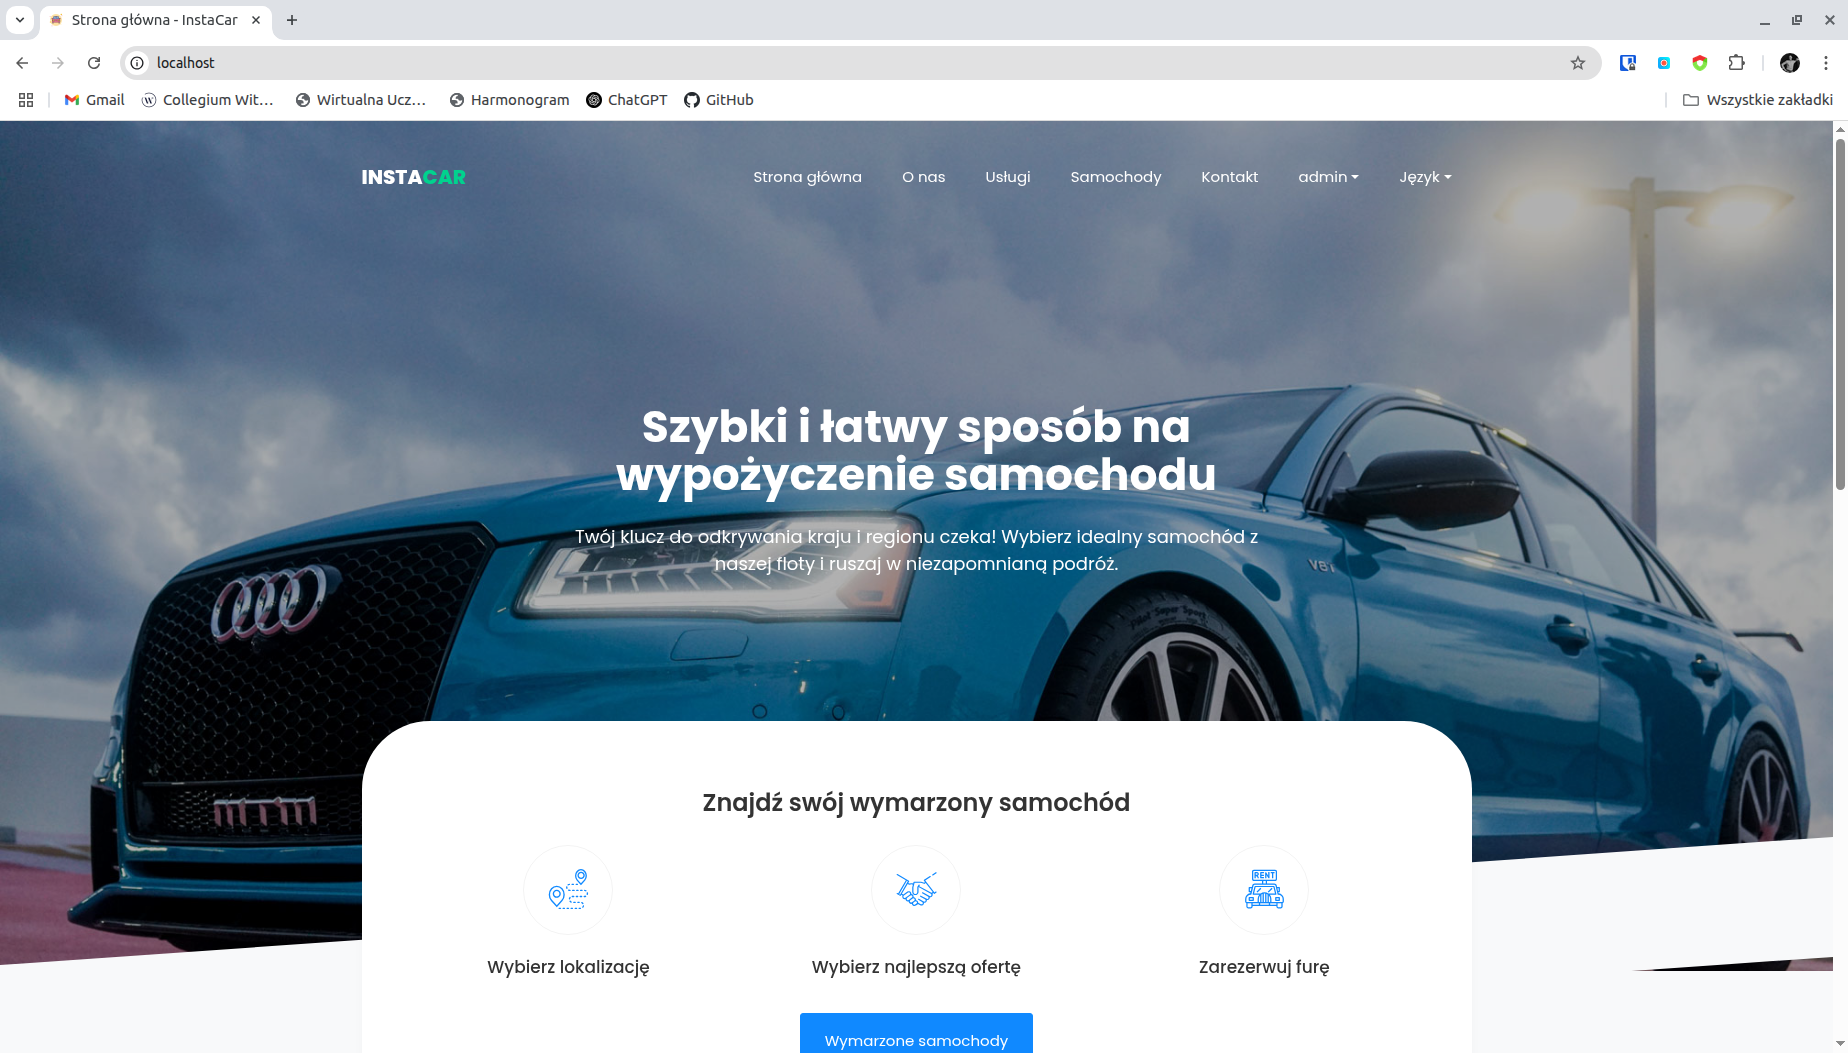
\includegraphics[width=1\linewidth]{homepage}
		\caption{Widok strony głównej}
		\label{fig:homepage}
	\end{figure}
	
	\begin{figure}[H]
		\centering
		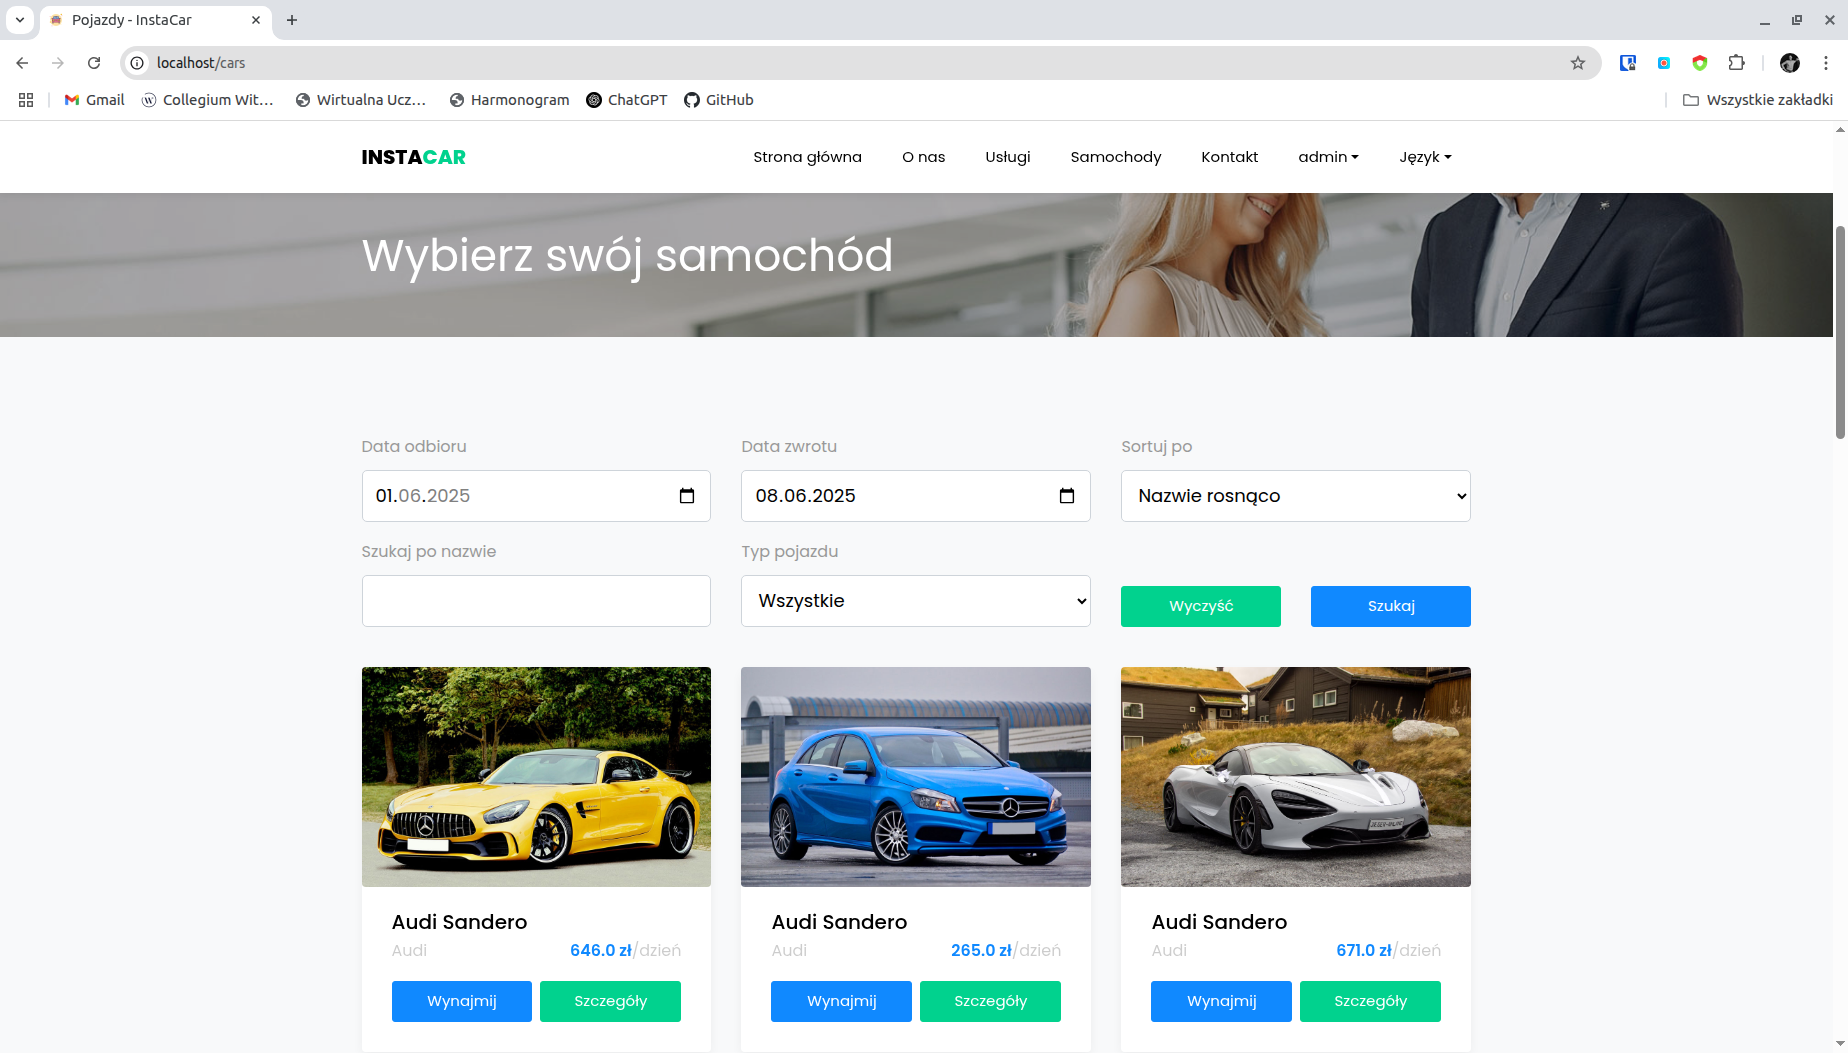
\includegraphics[width=1\linewidth]{cars}
		\caption{Widok wyboru samochodu}
		\label{fig:cars}
	\end{figure}
	
	\subsection{Widok administratora}
	
	Interfejs administratora dostępny jest po zalogowaniu się użytkownika z odpowiednimi uprawnieniami. Układ strony został podzielony na dwie główne części: panel nawigacyjny znajdujący się po lewej stronie oraz obszar roboczy po prawej.
	
	Panel boczny umożliwia szybki dostęp do kluczowych funkcjonalności systemu:
	
	\begin{itemize}
		\item \textbf{Strona główna} – ekran powitalny z podstawowymi informacjami,
		\item \textbf{Pojazdy} – zarządzanie bazą samochodów,
		\item \textbf{Zamówienia} – przegląd i edycja rezerwacji,
		\item \textbf{Użytkownicy} – zarządzanie kontami użytkowników,
		\item \textbf{Role} – wyświetlanie dostępnych ról i liczby przypisanych do nich użytkowników,
		\item \textbf{Powrót} – przejście do widoku użytkownika końcowego,
		\item \textbf{Wyloguj} – zakończenie sesji i wylogowanie z systemu.
	\end{itemize}
	
	W prawej części ekranu wyświetlana jest zawartość wybranej sekcji, umożliwiająca administratorowi wykonywanie odpowiednich operacji zarządczych.
	
	\begin{figure}[H]
		\centering
		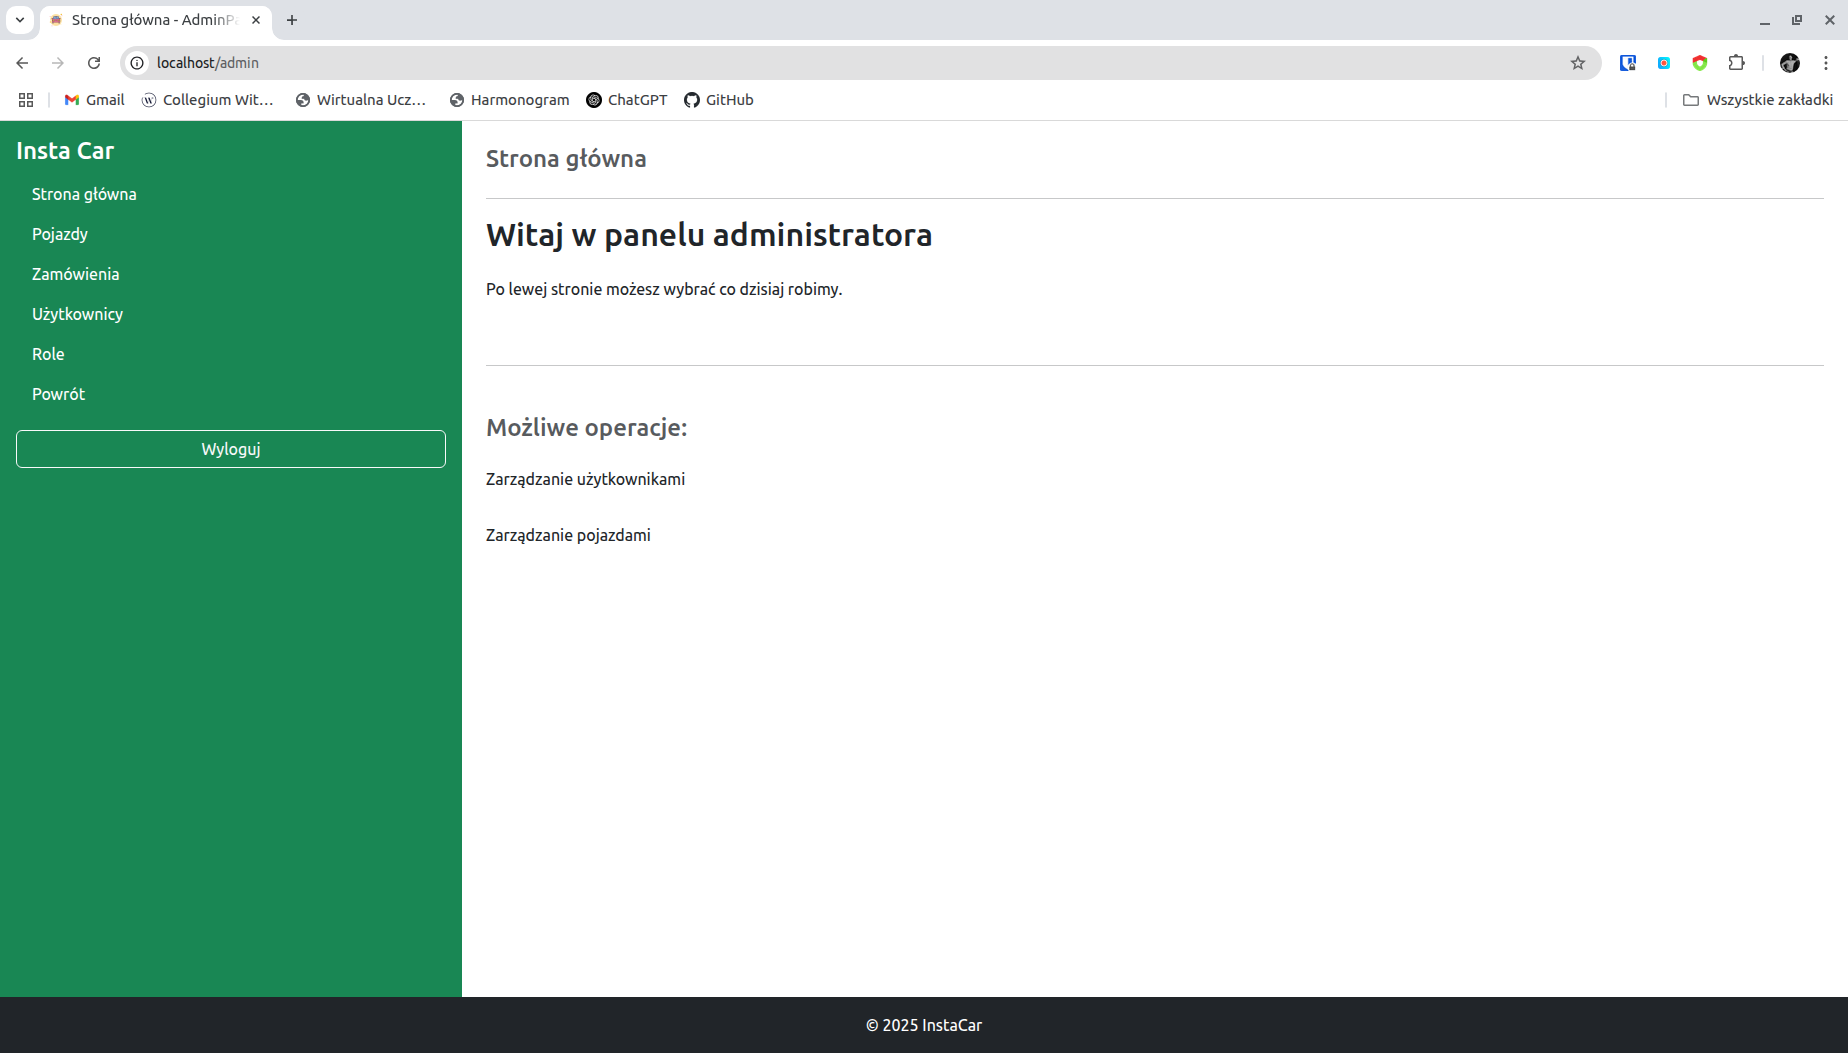
\includegraphics[width=1\linewidth]{admin_panel}
		\caption{Panel administracyjny – widok główny}
		\label{fig:admin_panel}
	\end{figure}
	
	\begin{figure}[H]
		\centering
		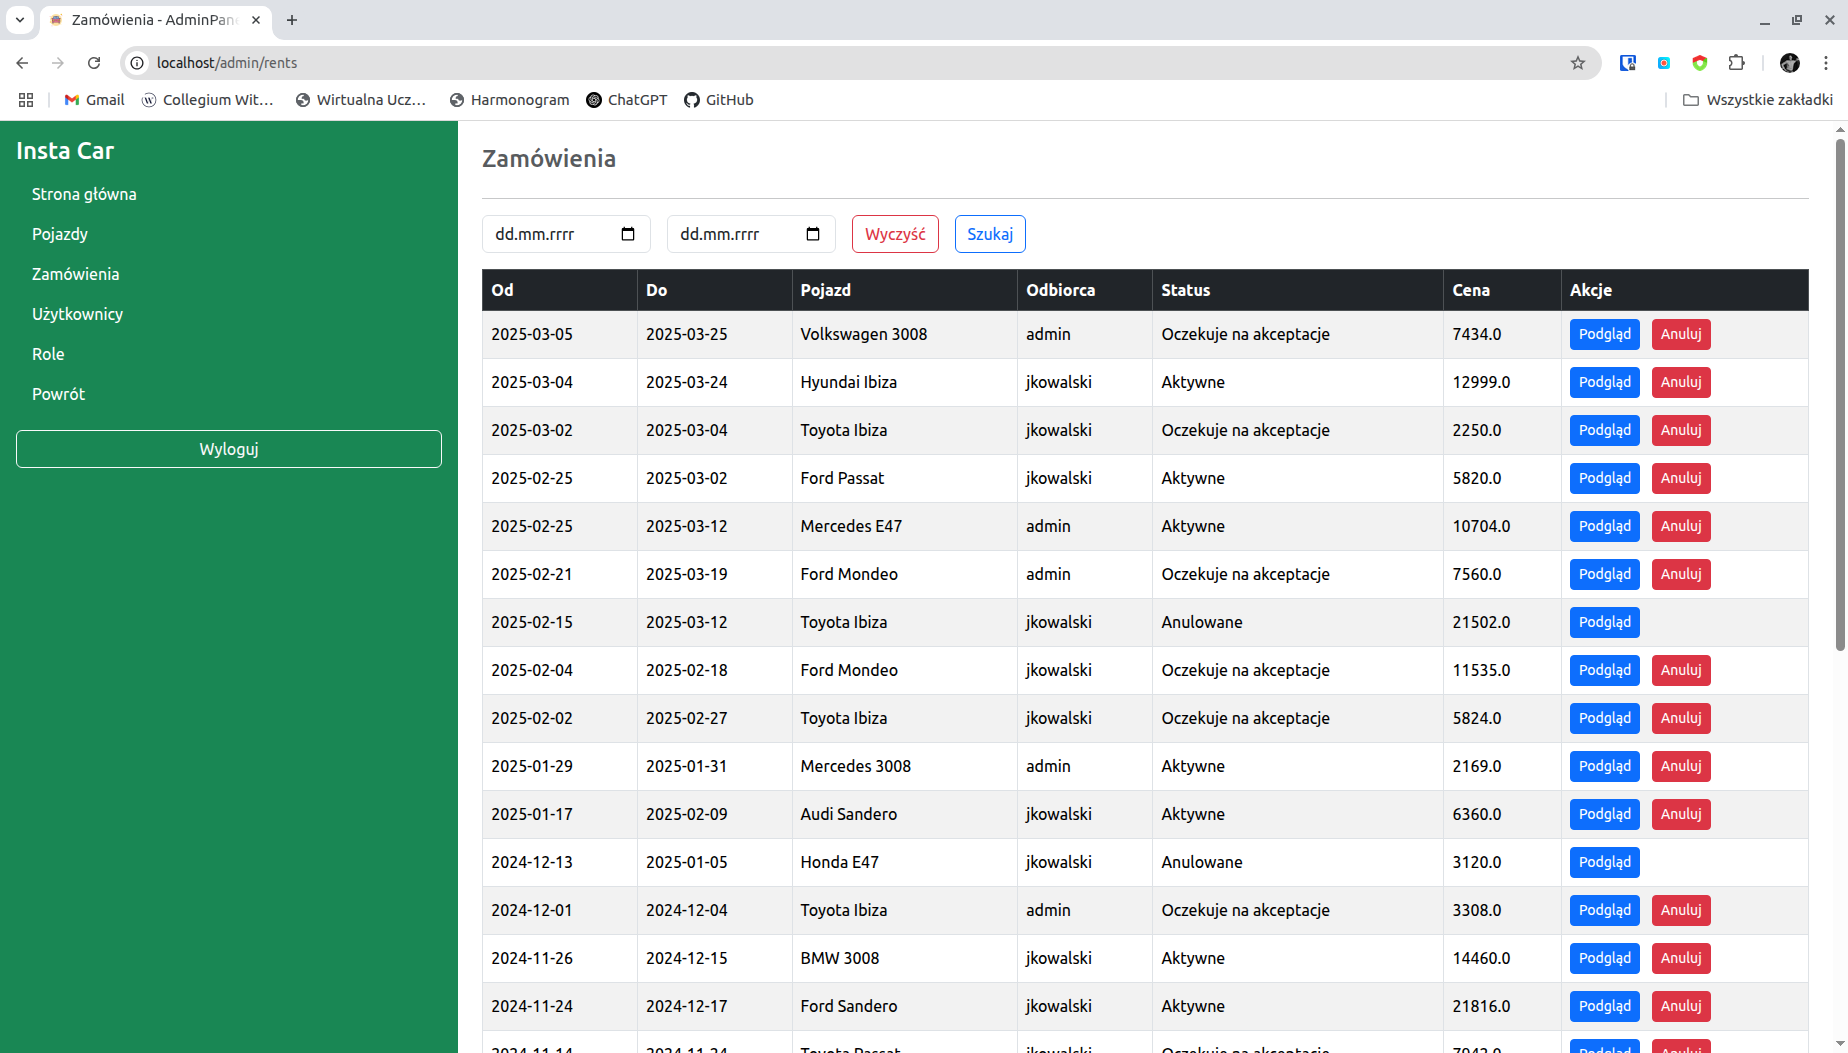
\includegraphics[width=1\linewidth]{zamowienia}
		\caption{Panel administracyjny – widok zamówień}
		\label{fig:zamowienia}
	\end{figure}
	
	
	\subsection{Styl wizualny i doświadczenie użytkownika (UX)}
	Projekt interfejsu użytkownika aplikacji został przygotowany z myślą o prostocie, przejrzystości oraz łatwości nawigacji. Główne założenia dotyczące stylu wizualnego oraz UX obejmują:
	\begin{itemize}
		\item \textbf{Minimalistyczny design} – zredukowana ilość elementów dekoracyjnych na rzecz funkcjonalności i czytelności treści.
		\item \textbf{Konsekwentna kolorystyka} – dominującym kolorem jest zieleń, stosowana w panelach bocznych, przyciskach i nagłówkach. Kolor ten jest używany także do wyróżniania aktywnych elementów nawigacyjnych.
		\item \textbf{Responsywny układ} – interfejs został zaprojektowany w sposób umożliwiający wygodne korzystanie zarówno na komputerach, jak i na urządzeniach mobilnych.
		\item \textbf{Intuicyjna nawigacja} – wszystkie kluczowe sekcje aplikacji są dostępne z poziomu głównego menu, dzięki czemu użytkownik zawsze wie, gdzie się znajduje i jak wrócić do wcześniejszych ekranów.
		\item \textbf{Powiadomienia i walidacja} – użytkownik jest na bieżąco informowany o wynikach swoich akcji (np. wysyłanie formularzy, błędy walidacyjne), co zwiększa poczucie kontroli nad systemem.
		\item \textbf{Zachowanie danych w formularzach} – w przypadku błędów formularzowych dane wprowadzone przez użytkownika nie są tracone, co znacząco poprawia komfort korzystania z~aplikacji.
	\end{itemize}
	Dzięki powyższym rozwiązaniom interfejs jest przyjazny dla użytkownika końcowego, a zarazem funkcjonalny i efektywny z punktu widzenia administratora systemu.
	
	\section{Dokumentacja technologiczna}
	\label{sec:dokumentacja_technologiczna}
	\subsection{Struktura bazy danych}
	Baza danych aplikacji do wynajmu samochodów została zaprojektowana tak, aby efektywnie zarządzać wszystkimi kluczowymi aspektami systemu -- od danych użytkowników i pojazdów, po szczegóły transakcji wynajmu. Poniżej przedstawiono przegląd głównych tabel i ich wzajemnych relacji:
	
	\subsubsection{\texttt{flyway\_schema\_history}}
	Ta tabela służy do śledzenia i zarządzania \textbf{wersjami schematu bazy danych} za pomocą narzędzia Flyway. Zawiera metadane o każdej zastosowanej migracji, takie jak wersja, opis, skrypt i~status wykonania.
	
	\subsubsection{\texttt{roles}}
	Definiuje \textbf{role użytkowników} w systemie (np. \texttt{ADMIN}, \texttt{USER}), co umożliwia zarządzanie uprawnieniami i dostępem.
	
	\subsubsection{\texttt{app\_users}}
	Centralna tabela przechowująca \textbf{informacje o kontach użytkowników}, w tym dane uwierzytelniające (nazwa użytkownika, e-mail, hasło) oraz odniesienie do ich roli w systemie. Obsługuje również różne metody uwierzytelniania, takie jak lokalne i przez zewnętrznych dostawców (np.~Google).
	
	\subsubsection{\texttt{email\_tokens} i \texttt{password\_tokens}}
	Te tabele są używane do zarządzania \textbf{tokenami weryfikacyjnymi} (dla adresów e-mail) oraz \textbf{tokenami do resetowania hasła}. Przechowują tokeny, ich status użycia i daty wygaśnięcia, zapewniając bezpieczeństwo procesów związanych z kontem.
	
	\subsubsection{\texttt{car\_models}}
	Zawiera ogólne \textbf{dane techniczne modeli samochodów}, takie jak marka, nazwa modelu, typ nadwozia, liczba miejsc, drzwi, rodzaj paliwa i skrzynia biegów. Jest to słownik modeli, na podstawie których później tworzone są konkretne pojazdy.
	
	\subsubsection{\texttt{vehicles}}
	Ta tabela przechowuje \textbf{szczegółowe informacje o poszczególnych pojazdach} dostępnych do wynajęcia. Każdy wpis odwołuje się do \texttt{car\_models} i zawiera unikalne dane, takie jak numer rejestracyjny, VIN, rok produkcji, kolor, cena wynajmu oraz adres URL do zdjęcia. Jest to tabela nadrzędna dla bardziej specyficznych typów pojazdów.
	
	\subsubsection{\texttt{city\_cars} i \texttt{sport\_cars}}
	Są to tabele dziedziczące po \texttt{vehicles}, przechowujące \textbf{dodatkowe atrybuty specyficzne dla danego typu pojazdu}. Na przykład \texttt{city\_cars} zawiera pojemność bagażnika, a \texttt{sport\_cars} moc silnika, przyspieszenie i prędkość maksymalną.
	
	\subsubsection{\texttt{user\_details}}
	Rozszerza informacje o użytkownikach, przechowując \textbf{szczegóły osobiste i kontaktowe}, takie jak imię, nazwisko, numer telefonu i adres.
	
	\subsubsection{\texttt{cities}}
	Lista \textbf{miast}, w których możliwy jest odbiór lub zwrot pojazdów.
	
	\subsubsection{\texttt{rents}}
	Kluczowa tabela do zarządzania \textbf{transakcjami wynajmu}. Rejestruje, kto wynajął pojazd, który pojazd, daty wynajmu, całkowity koszt, miejsca odbioru i zwrotu, a także status wynajmu.
	
	\subsection{Opis środowiska}
	\subsubsection{Baza danych - PostgreSQL 17.2}
	System bazodanowy wykorzystywany w projekcie to PostgreSQL w wersji 17.2. PostgreSQL to wydajny, stabilny i bezpieczny system zarządzania relacyjną bazą danych, szeroko stosowany w~środowiskach produkcyjnych. \\
	Konfiguracja dostępu do bazy danych znajduje się w pliku docker-compose.yml.
	
	\subsubsection{Migracje schematu – Flyway 10.20.1}
	Do zarządzania migracjami schematu bazy danych wykorzystywane jest narzędzie Flyway w wersji 10.20.1. Flyway umożliwia wersjonowanie zmian w strukturze bazy danych i ich automatyczne stosowanie w środowiskach deweloperskich, testowych oraz produkcyjnych. \\
	Cechy użycia Flyway w projekcie:
	\begin{itemize}
		\item migracje definiowane w postaci skryptów SQL w katalogu db/migration,
		
		\item automatyczne wykrywanie i stosowanie nowych migracji przy starcie aplikacji,
		
		\item wsparcie dla rollbacków i walidacji historii migracji.
	\end{itemize}
	
	\subsubsection{Cache – Redis 7.4.2-alpine}
	\label{cache}
	Do przechowywania danych tymczasowych oraz buforowania odpowiedzi system korzysta z Redis w wersji 7.4.2-alpine. Redis działa jako zewnętrzny, szybki magazyn danych typu key-value, wykorzystywany m.in. do cache’owania wyników zapytań i danych sesyjnych. \\
	Wersja alpine została wybrana ze względu na minimalny rozmiar obrazu oraz szybki czas uruchamiania kontenera.
	
	\section{Zagadnienia kwalifikacyjne}
	\subsection{Framework MVC}
	Projekt wykorzystuje framework Spring Boot, który implementuje wzorzec architektoniczny MVC (Model-View-Controller). Dzięki temu możliwe jest logiczne rozdzielenie warstwy danych (Model), interfejsu użytkownika (View) oraz logiki sterującej (Controller).\\
	W projekcie zastosowano m.in. startery Spring Boot:
	\begin{itemize}
		\item spring-boot-starter-web – do tworzenia warstwy webowej, obsługującej żądania HTTP
		\item spring-boot-starter-thymeleaf – jako silnik szablonów do generowania widoków HTML
		\item spring-boot-starter-security – do zarządzania uwierzytelnianiem i autoryzacją
		\item spring-boot-starter-data-jpa – do integracji warstwy modelu z bazą danych poprzez JPA (ORM).
	\end{itemize}
	Struktura aplikacji jest zgodna z koncepcją MVC, gdzie kontrolery odbierają zapytania od użytkownika, komunikują się z modelem (np. warstwą usług i repozytoriów bazodanowych) i zwracają odpowiednie widoki generowane przez Thymeleaf. Takie podejście ułatwia utrzymanie, testowanie i rozwój aplikacji.
	
	\subsection{Framework CSS}
	W projekcie zastosowano framework CSS \textbf{Bootstrap} w wersji 4.5.0, co pozwoliło na szybkie i efektywne tworzenie responsywnego i estetycznego interfejsu użytkownika. Bootstrap dostarcza gotowe komponenty, siatkę (grid system) oraz zestaw klas ułatwiających stylizację elementów strony bez konieczności pisania dużej ilości własnego kodu CSS. Wykorzystanie frameworka znacząco przyspieszyło proces implementacji oraz zapewniło spójny wygląd aplikacji na różnych urządzeniach i~rozdzielczościach.
	
	\subsection{Baza danych}
	Zagadnienie \textbf{baza danych} jest w pełni spełnione. Szczegółowy opis struktury bazy danych znajduje się w rozdziale ~\ref{sec:dokumentacja_technologiczna} – \nameref{sec:dokumentacja_technologiczna}.
	
	\subsection{Cache}
	Zagadnienie \textbf{cache} zostało w pełni zaimplementowane. W projekcie wykorzystano system Redis do buforowania danych i przyspieszania działania aplikacji. Szczegółowy opis konfiguracji oraz zastosowań pamięci podręcznej znajduje się w podrozdziale~\ref{cache} - \nameref{cache}.
	
	\subsection{Dependency manager}
	W projekcie zarządzanie zależnościami odbywa się za pomocą narzędzia Maven. Plik konfiguracyjny \texttt{pom.xml} zawiera wszystkie niezbędne zależności, takie jak Spring Boot, bazy danych (PostgreSQL, H2), biblioteki do bezpieczeństwa, szablonów Thymeleaf, obsługi maili, Redis oraz testów.\\
	Maven automatycznie pobiera i aktualizuje wymagane biblioteki, co ułatwia utrzymanie spójności wersji oraz integrację z innymi narzędziami. Dzięki temu proces budowania aplikacji jest zautomatyzowany i powtarzalny, a także umożliwia łatwe zarządzanie wersjami i rozszerzeniami projektu.
	
	\subsection{HTML}
	Struktura dokumentów HTML w aplikacji została przygotowana z myślą o czytelności i łatwej nawigacji. W celu zapewnienia responsywności oraz estetycznego wyglądu, szablony HTML wykorzystują klasy i komponenty frameworka Bootstrap w wersji 4.5, co umożliwia szybkie i spójne tworzenie układów strony, formularzy, przycisków oraz innych elementów interfejsu użytkownika.
	\begin{lstlisting}[language=HTML, caption={Kod HTML strony głównej}]
	<html lang="pl">
	<th:block th:replace="~{/fragments/headerFragments :: head(#{home.title})}"></th:block>
	<body>
	<th:block th:replace="~{/fragments/bodyFragments :: navbar}"></th:block>
	
	<div class="hero-wrap ftco-degree-bg" style="background-image: url('/images/bg_1.jpg');"
	data-stellar-background-ratio="0.5">
	<div class="overlay"></div>
	<div class="container">
	<div class="row no-gutters slider-text justify-content-start align-items-center justify-content-center">
	<div class="col-lg-8 ftco-animate">
	<div class="text w-100 text-center mb-md-5 pb-md-5">
	<h1 class="mb-4" th:text="#{home.header}"></h1>
	<p style="font-size: 18px;" th:text="#{home.subheader}"></p>
	</div>
	</div>
	</div>
	</div>
	</div>
	
	<section class="ftco-section ftco-no-pt bg-light">
	<div class="container">
	<div class="row no-gutters">
	<div class="col-md-12	featured-top">
	<div class="row no-gutters">
	<div class="col-md-12 d-flex align-items-center">
	<div class="services-wrap rounded-right rounded-left w-100 text-center">
	<h3 class="heading-section mb-4 text-center" th:text="#{home.text.main}"></h3>
	<div class="row d-flex mb-4">
	<div class="col-md-4 d-flex align-self-stretch ftco-animate">
	<div class="services w-100 text-center">
	<div class="icon d-flex align-items-center justify-content-center"><span class="flaticon-route"></span></div>
	<div class="text w-100">
	<h3 class="heading mb-2" th:text="#{home.text.location}"></h3>
	</div>
	</div>
	</div>
	<div class="col-md-4 d-flex align-self-stretch ftco-animate">
	<div class="services w-100 text-center">
	<div class="icon d-flex align-items-center justify-content-center"><span class="flaticon-handshake"></span></div>
	<div class="text w-100">
	<h3 class="heading mb-2" th:text="#{home.text.offer}"></h3>
	</div>
	</div>
	</div>
	<div class="col-md-4 d-flex align-self-stretch ftco-animate">
	<div class="services w-100 text-center">
	<div class="icon d-flex align-items-center justify-content-center"><span class="flaticon-rent"></span></div>
	<div class="text w-100">
	<h3 class="heading mb-2" th:text="#{home.text.rent}"></h3>
	</div>
	</div>
	</div>
	</div>
	<p><a th:href="@{/cars}" class="btn btn-primary py-3 px-4" th:text="#{home.submit}"></a></p>
	</div>
	</div>
	</div>
	</div>
	</div>
	</div>
	</section>
	<th:block th:replace="~{/fragments/bodyFragments :: services}"></th:block>
	<th:block th:replace="~{/fragments/bodyFragments :: footer}"></th:block>
	<th:block th:replace="~{/fragments/bodyFragments :: loader}"></th:block>
	<th:block th:replace="~{/fragments/bodyFragments :: scripts}"></th:block>
	</body>
	</html>
	\end{lstlisting}
	
	\subsection{CSS}
	Poza wykorzystaniem Bootstrapa, projekt zawiera również własne style CSS, które uzupełniają i~modyfikują wygląd interfejsu zgodnie z wymaganiami funkcjonalnymi i wizualnymi aplikacji. Style te obejmują dostosowanie kolorów, marginesów, fontów oraz drobne korekty elementów, których nie obsługuje Bootstrap domyślnie. Własny kod CSS jest dobrze zorganizowany i umieszczony w osobnych plikach, co ułatwia jego utrzymanie i rozwój projektu.
	\begin{lstlisting}[language=CSS, caption={Fragment kodu CSS}]
	html {
	font-family: sans-serif;
	line-height: 1.15;
	-webkit-text-size-adjust: 100%;
	-webkit-tap-highlight-color: rgba(0, 0, 0, 0); }
	
	article, aside, figcaption, figure, footer, header, hgroup, main, nav, section {
	display: block; }
	
	body {
	margin: 0;
	font-family: -apple-system, BlinkMacSystemFont, "Segoe UI", Roboto, "Helvetica Neue", Arial, "Noto Sans", sans-serif, "Apple Color Emoji", "Segoe UI Emoji", "Segoe UI Symbol", "Noto Color Emoji";
	font-size: 1rem;
	font-weight: 400;
	line-height: 1.5;
	color: #212529;
	text-align: left;
	background-color: #fff; }
	\end{lstlisting}
	
	\subsection{JavaScript}
	W projekcie JavaScript został wykorzystany głównie do obsługi interakcji na stronie frontendowej oraz działania komponentów z frameworka Bootstrap. Nie zastosowano dedykowanych frameworków JavaScript ani rozbudowanych skryptów. Implementacja opiera się na standardowych rozwiązaniach, które wspierają responsywność i podstawową dynamikę aplikacji.
	\begin{lstlisting}[style=jsStyle, caption={Fragment kodu JavaScript}]
	var isMobile = {
	Android: function() {
	return navigator.userAgent.match(/Android/i);
	},
	BlackBerry: function() {
	return navigator.userAgent.match(/BlackBerry/i);
	},
	iOS: function() {
	return navigator.userAgent.match(/iPhone|iPad|iPod/i);
	},
	Opera: function() {
	return navigator.userAgent.match(/Opera Mini/i);
	},
	Windows: function() {
	return navigator.userAgent.match(/IEMobile/i);
	},
	any: function() {
	return (
	isMobile.Android() ||
	isMobile.BlackBerry() ||
	isMobile.iOS() ||
	isMobile.Opera() ||
	isMobile.Windows()
	);
	}
	};
	\end{lstlisting}
	
	\subsection{Routing}
	Routing w projekcie realizowany jest za pomocą frameworka Spring Boot. Żądania HTTP są mapowane na odpowiednie metody kontrolerów przy użyciu adnotacji takich jak \texttt{@GetMapping} czy \texttt{@PostMapping}. Dzięki temu możliwe jest czytelne i efektywne zarządzanie ścieżkami URL oraz obsługa różnych metod HTTP.
	
	\subsection{ORM}
	Zagadnienie \textbf{ORM} zostało zrealizowane przy użyciu warstwy mapowania obiektowo-relacyjnego, która pozwala na bezpośrednie odwzorowanie klas w aplikacji na tabele w bazie danych. Dzięki temu możliwa jest wygodna i bezpieczna manipulacja danymi bez konieczności pisania zapytań SQL. ORM obsługuje relacje między encjami, dziedziczenie oraz walidację danych.
	
	\subsection{Uwierzytelnienie}
	Zagadnienie \textbf{uwierzytelnienie} zostało w pełni zaimplementowane. System umożliwia logowanie lokalne oraz za pomocą zewnętrznych dostawców (np. Google). Dane uwierzytelniające są przechowywane w tabeli \texttt{app\_users}, a dodatkowe mechanizmy bezpieczeństwa, takie jak tokeny resetowania hasła i potwierdzania adresu e-mail, zostały zaimplementowane z użyciem tabel \texttt{email\_tokens} i \texttt{password\_tokens}.
	
	\subsection{Lokalizacja}
	W projekcie zaimplementowano mechanizm lokalizacji umożliwiający wybór języka polskiego lub angielskiego. Teksty w aplikacji są przechowywane w plikach \texttt{messages\_en.properties} oraz \texttt{messages\_pl.properties}, które odpowiadają poszczególnym wersjom językowym. Dzięki temu aplikacja dynamicznie dostosowuje się do preferencji użytkownika, wyświetlając treści w wybranym języku.
	
	\subsection{Mailing}
	Zagadnienie \textbf{mailing} zostało zrealizowane poprzez wysyłanie wiadomości e-mail służących m.in.~do weryfikacji konta i resetowania hasła. System generuje unikalne tokeny, które są przesyłane użytkownikom w wiadomościach zawierających odpowiednie linki aktywacyjne lub resetujące.
	
	\subsection{Formularze}
	W aplikacji formularze występują w różnych miejscach – zarówno po stronie użytkownika końcowego, jak i w panelu administracyjnym. Służą one do obsługi różnorodnych operacji, takich jak rejestracja, logowanie, składanie zamówień, dodawanie produktów, edycja danych i wiele innych funkcjonalności systemu. \\
	Do tworzenia formularzy wykorzystano silnik szablonów Thymeleaf, który umożliwia łatwe powiązanie elementów formularza z danymi modelu oraz wspiera integrację z mechanizmem walidacji Spring Boota. Po wysłaniu danych formularzowych, są one przekazywane do odpowiedniego kontrolera w warstwie backendowej, gdzie poddawane są szczegółowej walidacji (zarówno po stronie klienta, jak i serwera).\\
	W przypadku wykrycia błędów walidacyjnych (np. brak wymaganych pól, nieprawidłowy format danych), użytkownikowi wyświetlane są odpowiednie komunikaty o błędach, bez konieczności ponownego wypełniania całego formularza – dane wprowadzone przez użytkownika są zachowywane i~ponownie wyświetlane w formularzu. Dzięki temu rozwiązaniu użytkownik może szybko poprawić błędne dane, co znacząco wpływa na wygodę obsługi interfejsu i użyteczność aplikacji.
	\begin{figure}[H]
		\centering
		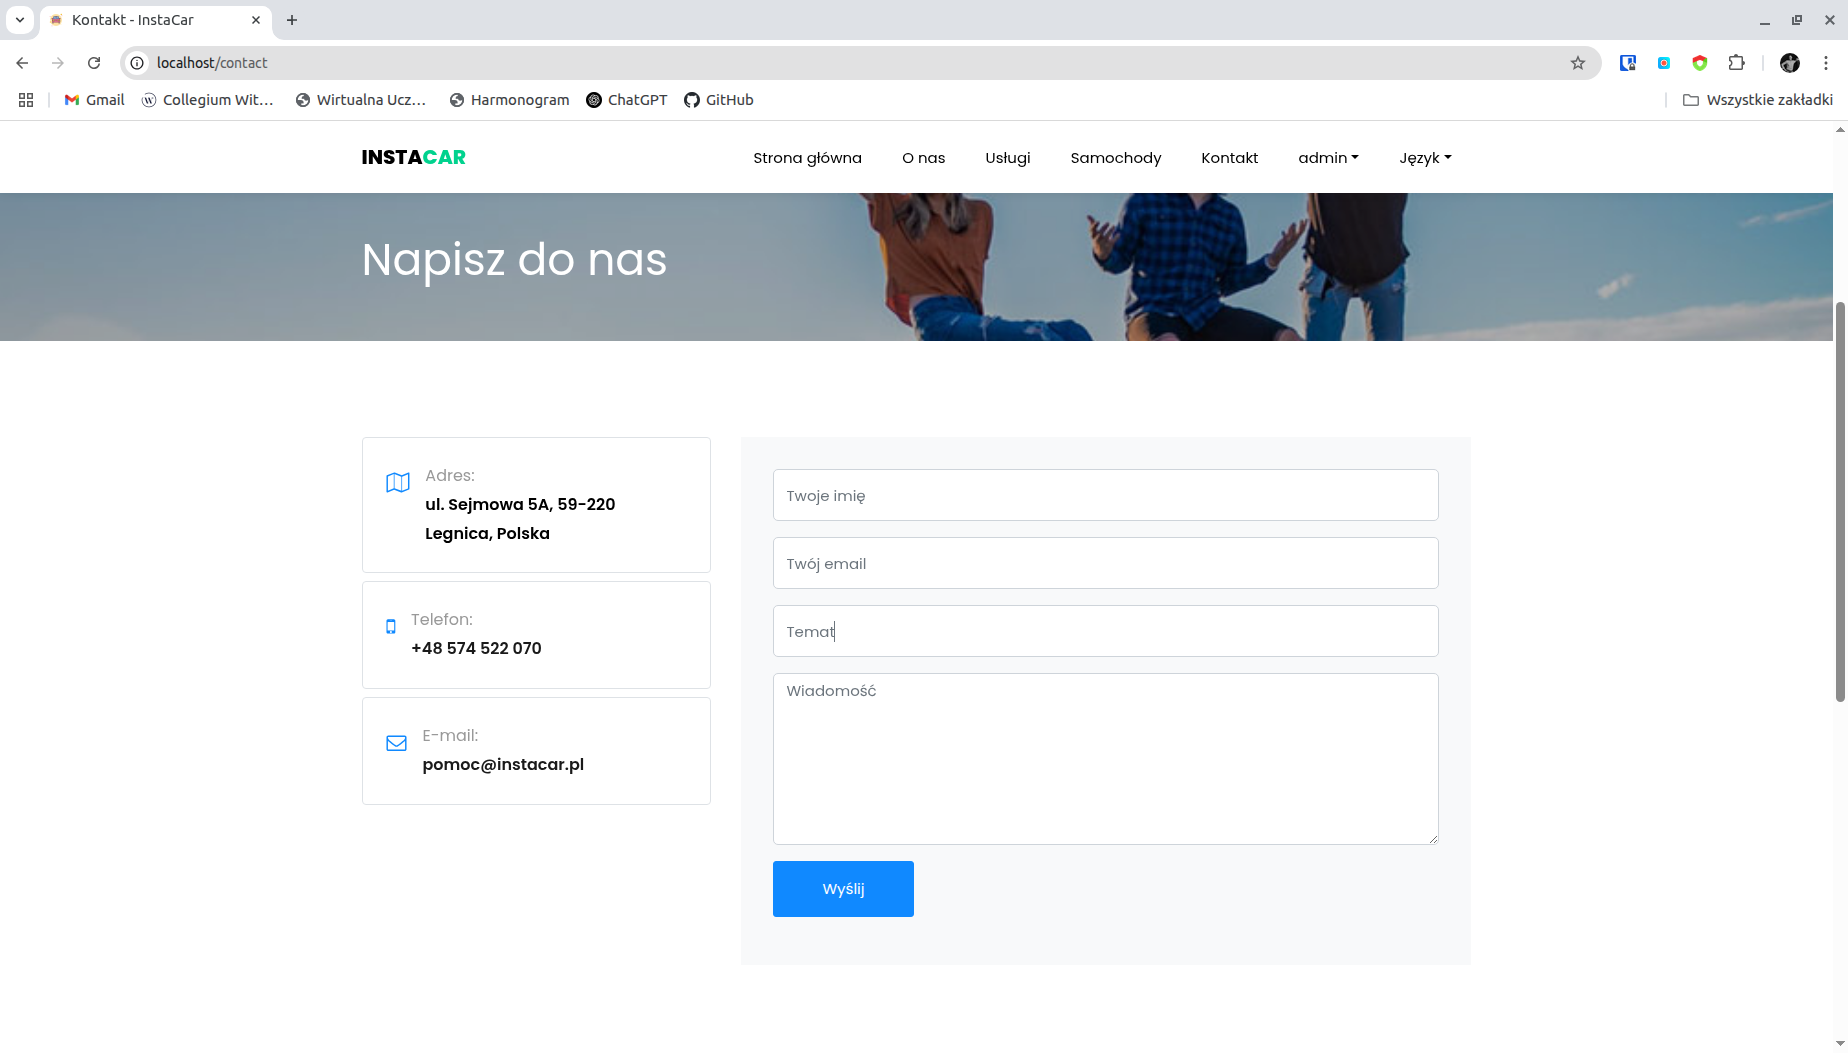
\includegraphics[width=1\linewidth]{formularz}
		\caption{Formularz kontaktowy}
		\label{fig:formularz}
	\end{figure}
	
	\subsection{Asynchroniczne interakcje}
	Zagadnienie \textbf{asynchronicznych interakcji} nie zostało zaimplementowane w obecnej wersji aplikacji. Wszystkie operacje realizowane są w sposób synchroniczny.
	
	\subsection{Konsumpcja API}
	Projekt wykorzystuje mechanizmy komunikacji z zewnętrznymi API, co umożliwia pobieranie i~przetwarzanie danych spoza aplikacji. Dzięki temu system może integrować się z innymi serwisami i rozszerzać swoją funkcjonalność. W ramach konsumpcji API, aplikacja pobiera aktualne kursy walut bezpośrednio z Narodowego Banku Polskiego (NBP), co zapewnia dostęp do wiarygodnych i zawsze aktualnych danych.
	
	\subsection{Publikacja API}
	Aplikacja udostępnia własne API oparte na architekturze REST, które pozwala na zdalny dostęp do danych i funkcji systemu. Implementacja opiera się na frameworku Spring Boot, który zapewnia wygodne narzędzia do tworzenia i zabezpieczania endpointów. W ramach tego API, publikujemy dane dotyczące pojazdów oraz modeli samochodów, umożliwiając innym systemom łatwy dostęp i integrację z naszą bazą danych.
	
	\subsection{RWD}
	Interfejs aplikacji jest responsywny i dostosowuje się do różnych rozmiarów ekranów, zapewniając poprawne wyświetlanie i użyteczność na urządzeniach mobilnych, tabletach oraz komputerach stacjonarnych. W projekcie wykorzystano framework Bootstrap, który znacząco ułatwia tworzenie responsywnych layoutów.
	
	\subsection{Logger}
	W projekcie zastosowano mechanizmy logowania zdarzeń i błędów, które pomagają w monitorowaniu działania aplikacji oraz diagnozowaniu problemów. Logi są konfigurowane i zapisywane zgodnie z najlepszymi praktykami Spring Boot, co umożliwia łatwą analizę działania systemu.
	
	\subsection{Deployment}
	Zagadnienie \textbf{deployment} zostało zrealizowane z wykorzystaniem kontenerów Docker, co umożliwia łatwe wdrożenie aplikacji w różnych środowiskach. Cała konfiguracja usług (baza danych PostgreSQL, Redis, backend, frontend) znajduje się w pliku \texttt{docker-compose.yml}, co pozwala na szybkie uruchomienie całego systemu.
	
	\newpage
	\addcontentsline{toc}{section}{Spis rysunków}
	\listoffigures
	
	\addcontentsline{toc}{section}{Spis listingów}
	\lstlistoflistings
	
\end{document}